
\documentclass[sigconf]{acmart}
\usepackage{graphicx}
\usepackage{enumerate}

%%
%% \BibTeX command to typeset BibTeX logo in the docs
\AtBeginDocument{%
	\providecommand\BibTeX{{%
			\normalfont B\kern-0.5em{\scshape i\kern-0.25em b}\kern-0.8em\TeX}}}

%% Rights management information.  This information is sent to you
%% when you complete the rights form.  These commands have SAMPLE
%% values in them; it is your responsibility as an author to replace
%% the commands and values with those provided to you when you
%% complete the rights form.
\setcopyright{acmcopyright}
\copyrightyear{2018}
\acmYear{2018}
\acmDOI{10.1145/1122445.1122456}

%% These commands are for a PROCEEDINGS abstract or paper.
\acmConference[Woodstock '18]{Woodstock '18: ACM Symposium on Neural
	Gaze Detection}{June 03--05, 2018}{Woodstock, NY}
\acmBooktitle{Woodstock '18: ACM Symposium on Neural Gaze Detection,
	June 03--05, 2018, Woodstock, NY}
\acmPrice{15.00}
\acmISBN{978-1-4503-XXXX-X/18/06}


\begin{document}
	
	\title{Improving open domain question answering with Knowledge Base and Wikipedia graph}
	
	\author{Ruiyu Lin}
	\affiliation{%
		\institution{SUN YAT-SEN UNIVERSITY}}
	\email{linry23@mail2.sysu.edu.cn}
	
	
	\begin{abstract}
		A clear and well-documented \LaTeX\ document is presented as an
		
	\end{abstract}

	\keywords{ neural networks}

	\maketitle
	
	\section{Introduction}
	
	\textbf{Input}
		\begin{itemize}
			\item {Dataset}:(question, answer) pair.
			
			\item{ Knowledge Base}:(entity, relation, entity) triple.
			 Knowledge Base is a multi-relational graphs, each edge has a label and direction associated with it. Each node in the graph is an entity.
			 
			 \item{ Wikipedia graph\cite{asai2019learning}}:(text, text) pair.
			 Wikipedia graph is constructed by Hyperlinks and within-document links, Each node in the graph is an article.
				
		\end{itemize}
		

	\textbf{Output}
	representation of all the retrieved passage, as the input to a reader model to extract answer.
	
	\textbf{Goal} 
	To better embed the retrieved passage, which based on Wikipedia graph, with  Knowledge Base knowledge.
	
	\textbf{Method} 
	Fuse Knowledge Base knowledge into Wikipedia graph to formulate
	($\MakeUppercase{p}_{a}$, relation, $\MakeUppercase{p}_{b}$) triple.
	\begin{enumerate}[(1)]
		
		\item identify the relations between two passage node
		
		Assuming that :
		
		
		$rSet_{(a,b)}$ : the set of relation between $\MakeUppercase{p}_a$ and $\MakeUppercase{p}_b$, initialized empty
		
		($\MakeUppercase{p}_a$, 	$\MakeUppercase{p}_b$) exits in Wikipedia graph.
		
		
		$\MakeUppercase{p}_a$ contains n entities( $e_{a1},...,e_{an}$) ,
		
		$\MakeUppercase{p}_b$ contains m entities( $e_{b1},...,e_{bm}$) 
		
		
		If $(e_{ai}, r, e_{bj})$(1<=i,j<=n) exits in Knowledge Base, add r into $rSet_{(a,b)}$ . Finally, $rSet_{a,b} = (r_{1}...,r_{k}) $
		
		\item corperate identified relations into passage node embedding
		\begin{displaymath}
			\begin{aligned}
			\alpha_{r_i} = sorce( h_{a},e_{ai},r_i,q) \\
			h_{inter-b}= FNN (h_{a}, \sum_{i=1}^{k} \alpha_{r_i}*ri)
			\end{aligned}
		\end{displaymath}
		$h_{inter-b}$ is the intermediate representation of passage b.
		$\alpha_{r_i}$ is the relation score.
	
		Suppose that  $h_{b}$ is link by  $[h_{a1},...,h_{at}]$ ,then update $h_{b}$ by 
		\begin{displaymath}
			\begin{aligned}
				h_{b}= GCN(h_{b}, \sum_{1}^{t} h_{inter-b})
			\end{aligned}
		\end{displaymath}

	
	\item answer extraction
	
	We adopt Multi-passage BERT \cite{2019Multi} as our reader model,which use Shared normalization\cite{2018Simple}, specifically to process passages independently, but compute the span probability across spans in all passages in every mini-batch.Globally normalizing answer scores across all passages of the same question enables to find better answers by utilizing more passages.
	
	Denote the passage score as $Pr(P_i|Q, P)$,which reranks all retrieved passages
		\begin{displaymath}
			Pr(P_i|Q, P) = softmax(h_i^\mathrm{ T }  W)
		\end{displaymath}
			
	W is a trainable parameter.
	
	The score of an answer span from passage $\MakeUppercase{p}_i$ will be
			\begin{displaymath}
			Pr(a| Q, P) = 	Pr(P_i|Q, P)P_s(a_s|Q, P)P_e(a_e|Q, P).
			\end{displaymath}
	
		
		
		
	\end{enumerate} 
   
   	\textbf{Some details remain specific}
   	
   	\begin{enumerate}[(1)]
   		
   	\item how to get the representation of relation.
   	
	   	In GRAFT-Nets\cite{sun2018open}, they average word
	   	vectors to compute a relation vector  from the
	   	surface form of the relation.
	   	
	   	In PullNet\cite{sun2019pullnet} ,embedding of  relations are pretrained ,and can be looked up from an embedding table.
	   	
	   	In \cite{min2019knowledge} ,they only consider the most frequent 100 relations, and pretrain their embedding.	
	   	
	   	 \cite{xiong2019improving} tokenize the relation ,and then  encode it by a shared LSTM with the question .
	   
	   	
	   	In \cite{2020Composition},it handles multi-relational graphs  representation where each edge has a label and direction associated with it, and jointly embeds both nodes and relations in a relational graph.
	   	
	   	\begin{figure*}[ht]		
	   		\centering
	   		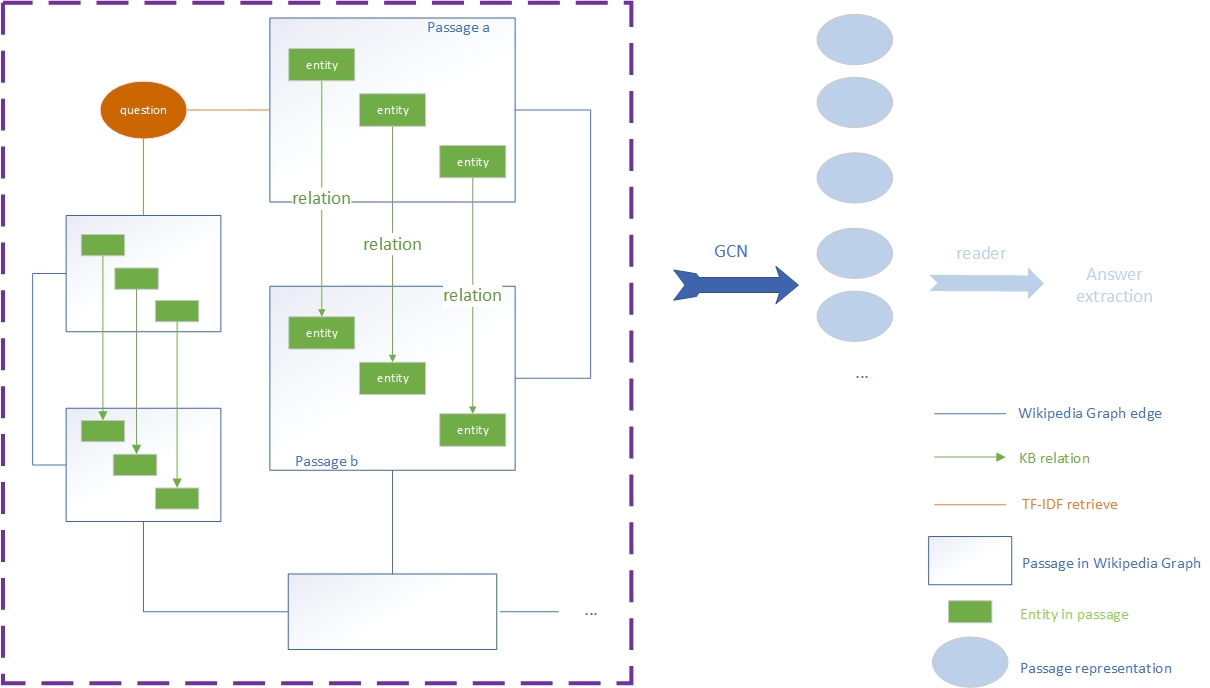
\includegraphics[scale=0.5]{model.jpg}
	   		\caption{A diagram of approach}
	   		\label{fig:label}
	   	\end{figure*}
	   	
   	
   	\item the representaion of question
   	
   		In GRAFT-Nets\cite{sun2018open},
   		the question representation is updated as
   		$h_q = FFN(\sum_{v\in S_q}h_v)$
   		, where $S_q$ denotes the seed entities mentioned in the question.
   		
   		In PullNet\cite{sun2019pullnet}and \cite{xiong2019improving} ,	the question representation is accquired by a LSTM.
   		
   		In \cite{min2019knowledge} ,the question is not directly encoded,but with passage jointly by BERT.
   		
   		
   	
   	
   	\item how to score relation attention
   	
	   	Most work take the dot product between the embedding of relation and question.Considering the different framework here,we reformulate the score as:
	   	 
	   	 \begin{displaymath}
	   	 	\begin{aligned}
	   	 		&\alpha_{r_i} = sorce( h_{a},e_{ai},r_i,q)    	 		
	   	 	\end{aligned}
	   	 \end{displaymath}
	     	
   \end{enumerate} 


	
	%%
	%% The next two lines define the bibliography style to be used, and
	%% the bibliography file.
	\bibliographystyle{ACM-Reference-Format}
	\bibliography{refs}
	
	
	
\end{document}
\endinput
%%
%% End of file `sample-sigconf.tex'.
